% !TEX root = ../../../main.tex
% 来源：中学数学实验教材·第一册（代数）
% 章节：因式分解与余式定理 / 辗转相除法
% 原始文件：5.tex，行 2280-2303
% 类型：tikz
% ---
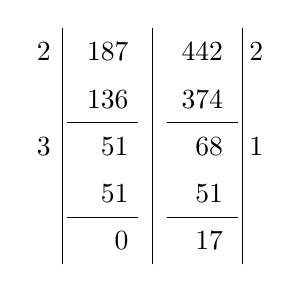
\begin{tikzpicture}[scale=.6]
\foreach \y/\ytext in {0/0,1/51,2/51,3/136,4/187}
{
    \node at (-1, \y)[left]{$\ytext$};
}    
\foreach \y/\ytext in {0/\boxed{17},1/51,2/68,3/374,4/442}
{
    \node at (1, \y)[left]{$\ytext$};
}   
\foreach \x in {-2.6,-.7,1.2}
{
    \draw (\x,-.5)--(\x,4.5);
}

\foreach \y in {.5, 2.5}
{
    \draw (-2.5,\y)--(-1,\y);
    \draw (-.4,\y)--(1.1,\y);
}
\node at (-3, 4) {2};
\node at (-3, 2) {3};
\node at (1.5, 4) {2};
\node at (1.5, 2) {1};
\end{tikzpicture}
